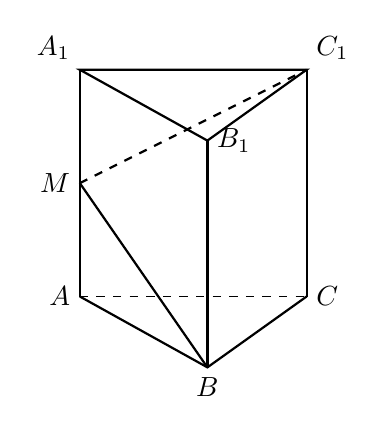
\begin{tikzpicture}[>=stealth, scale=0.9]
  % 顶点坐标
  \coordinate (A) at (0, 0);
  \coordinate (B) at (1.8, -1.0);
  \coordinate (C) at (3.2, 0);
  \coordinate (A1) at (0, 3.2);
  \coordinate (B1) at (1.8, 2.2);
  \coordinate (C1) at (3.2, 3.2);

  % AA1 上的交点 M
  \coordinate (M) at (0, 1.6);

  % 虚线（底面后边 AC 与后侧连线 MC1）
  \draw[dashed, thin] (A) -- (C);
  \draw[dashed, thick] (M) -- (C1);

  % 可见实线（棱与面）
  \draw[thick] (A) -- (B) -- (C);
  \draw[thick] (A1) -- (B1) -- (C1) -- cycle;
  \draw[thick] (A) -- (A1);
  \draw[thick] (B) -- (B1);
  \draw[thick] (C) -- (C1);

  % 折线路径的前半段 BM
  \draw[thick] (B) -- (M);

  % 顶点标签
  \node[left] at (A) {$A$};
  \node[below] at (B) {$B$};
  \node[right] at (C) {$C$};
  \node[left] at (M) {$M$};
  \node[above left] at (A1) {$A_1$};
  \node[right] at (B1) {$B_1$};
  \node[above right] at (C1) {$C_1$};
\end{tikzpicture}
